\documentclass[aspectratio=169]{../latex_main/tntbeamer}  % you can pass all options of the beamer class, e.g., 'handout' or 'aspectratio=43'
\usepackage{dsfont}
\usepackage{bm}
\usepackage[english]{babel}
\usepackage[T1]{fontenc}
%\usepackage[utf8]{inputenc}
\usepackage{graphicx}
\graphicspath{ {./figures/} }
\usepackage{algorithm}
\usepackage[ruled,vlined,algo2e,linesnumbered]{algorithm2e}
\usepackage{hyperref}
\usepackage{booktabs}
\usepackage{mathtools}

\usepackage{amsmath,amssymb}

\DeclareMathOperator*{\argmax}{arg\,max}
\DeclareMathOperator*{\argmin}{arg\,min}

\usepackage{amsbsy}
\newcommand{\vect}[1]{\bm{#1}}
%\newcommand{\vect}[1]{\boldsymbol{#1}}

\usepackage{pgfplots}
\pgfplotsset{compat=1.16}
\usepackage{tikz}
\usetikzlibrary{trees} 
\usetikzlibrary{shapes.geometric}
\usetikzlibrary{positioning,shapes,shadows,arrows,calc,mindmap}
\usetikzlibrary{positioning,fadings,through}
\usetikzlibrary{decorations.pathreplacing}
\usetikzlibrary{intersections}
\pgfdeclarelayer{background}
\pgfdeclarelayer{foreground}
\pgfsetlayers{background,main,foreground}
\tikzstyle{activity}=[rectangle, draw=black, rounded corners, text centered, text width=8em]
\tikzstyle{data}=[rectangle, draw=black, text centered, text width=8em]
\tikzstyle{myarrow}=[->, thick, draw=black]

% Define the layers to draw the diagram
\pgfdeclarelayer{background}
\pgfdeclarelayer{foreground}
\pgfsetlayers{background,main,foreground}

% Requires XeLaTeX or LuaLaTeX
%\usepackage{unicode-math}

\usepackage{fontspec}
%\setsansfont{Arial}
\setsansfont{RotisSansSerifStd}[ 
Path=../latex_main/fonts/,
Extension = .otf,
UprightFont = *-Regular,  % or *-Light
BoldFont = *-ExtraBold,  % or *-Bold
ItalicFont = *-Italic
]
\setmonofont{Cascadia Mono}[
Scale=0.8
]

% scale factor adapted; mathrm font added (Benjamin Spitschan @TNT, 2021-06-01)
%\setmathfont[Scale=1.05]{Libertinus Math}
%\setmathrm[Scale=1.05]{Libertinus Math}

% other available math fonts are (not exhaustive)
% Latin Modern Math
% XITS Math
% Libertinus Math
% Asana Math
% Fira Math
% TeX Gyre Pagella Math
% TeX Gyre Bonum Math
% TeX Gyre Schola Math
% TeX Gyre Termes Math

% Literature References
\newcommand{\lit}[2]{\href{#2}{\footnotesize\color{black!60}[#1]}}

%%% Beamer Customization
%----------------------------------------------------------------------
% (Don't) Show sections in frame header. Options: 'sections', 'sections light', empty
\setbeamertemplate{headline}{empty}

% Add header logo for normal frames
\setheaderimage{
	% 
\includegraphics[height=\logoheight]{figures/TNT_darkv4.pdf}
	
\includegraphics[height=\logoheight]{../latex_main/figures/luh_logo_rgb_0_80_155.pdf}
	% 
\includegraphics[height=\logoheight]{figures/logo_tntluh.pdf}
}

% Header logo for title page
\settitleheaderimage{
	% 
\includegraphics[height=\logoheight]{figures/TNT_darkv4.pdf}
	
\includegraphics[height=\logoheight]{../latex_main/figures/luh_logo_rgb_0_80_155.pdf}
	% 
\includegraphics[height=\logoheight]{figures/logo_tntluh.pdf}
}

% Title page: tntdefault 
\setbeamertemplate{title page}[tntdefault]  % or luhstyle
% Add optional title image here
%\addtitlepageimagedefault{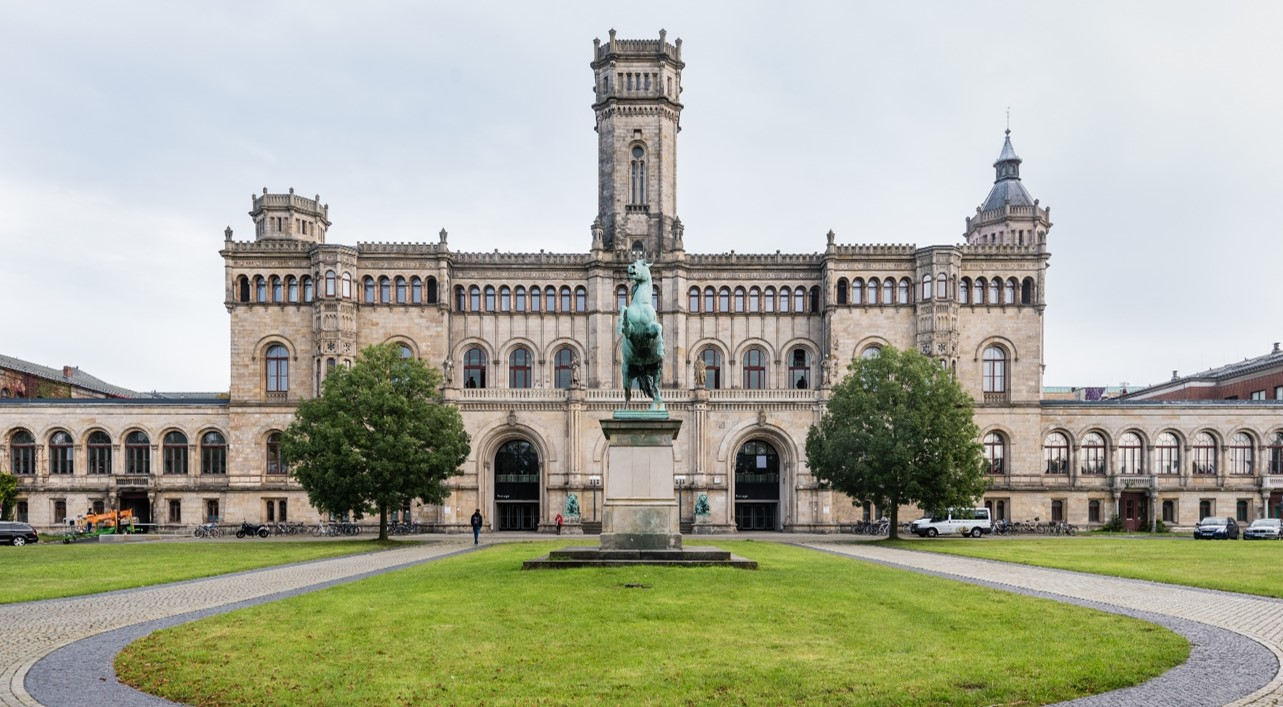
\includegraphics[width=0.65\textwidth]{figures/luh_default_presentation_title_image.jpg}}

% Title page: luhstyle
% \setbeamertemplate{title page}[luhstyle]
% % Add optional title image here
% \addtitlepageimage{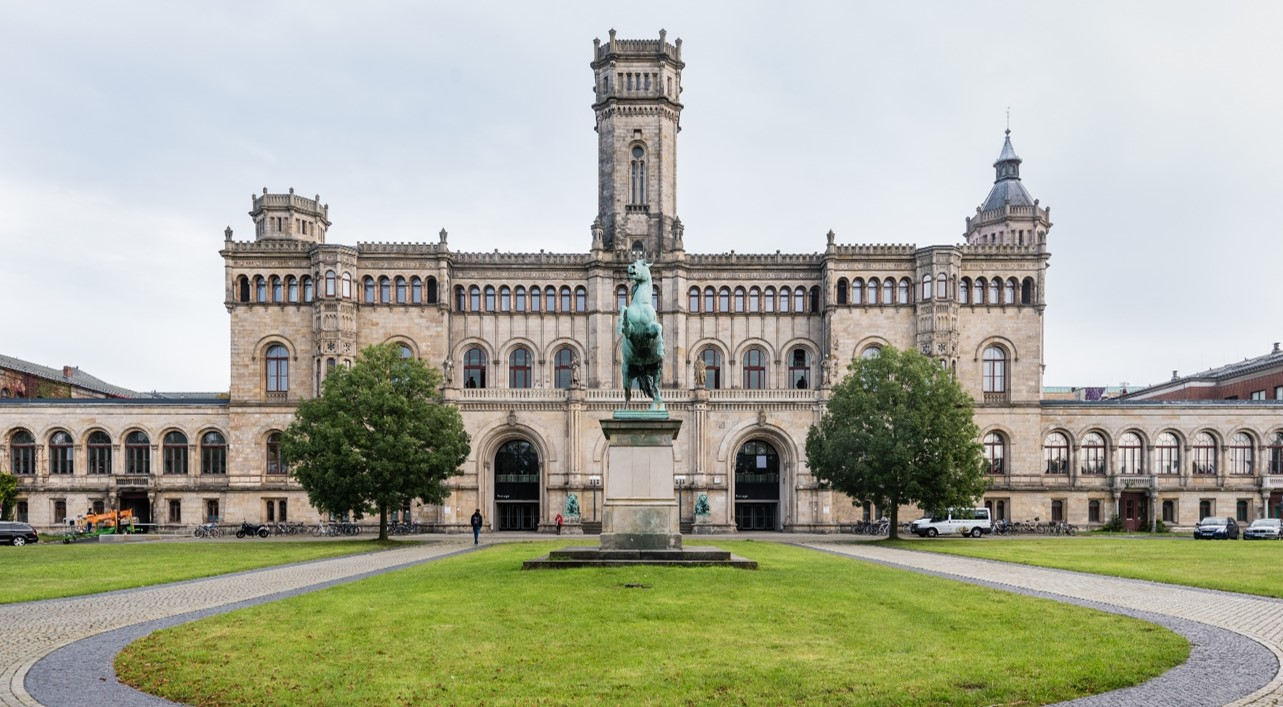
\includegraphics[width=0.75\textwidth]{figures/luh_default_presentation_title_image.jpg}}

\author[Abedjan \& Lindauer]{Ziawasch Abedjan \& Marius Lindauer\\[1em]
	
\includegraphics[height=\logoheight]{../latex_main/figures/luh_logo_rgb_0_80_155.pdf}\qquad
	
\includegraphics[height=\logoheight]{../latex_main/figures/DBIS_Kurzlogo.png}\qquad

\includegraphics[height=\logoheight]{../latex_main/figures/TNT_darkv4}\qquad

\includegraphics[height=\logoheight]{../latex_main/figures/L3S.jpg}	}
\date{Summer Term 2022; \hspace{0.5em} {
\includegraphics[height=1.5em]{../latex_main/figures/Cc-by-nc-sa_icon.svg.png}}; based on \href{https://ds100.org/fa21/}{[DS100]}
}


%%% Custom Packages
%----------------------------------------------------------------------
% Create dummy content
\usepackage{blindtext}

% Adds a frame with the current page layout. Just call \layout inside of a frame.
\usepackage{layout}


%%% Macros
%\renewcommand{\vec}[1]{\mathbf{#1}}
% \usepackage{bm}
%\let\vecb\bm

\title[Introduction]{DS: Logistic Regression, Classification}
\subtitle{Thresholding}

\graphicspath{ {./figure/} }
%\institute{}


\begin{document}
	
	\maketitle
	\begin{frame}{Classification}
	    Our motivation for performing logistic regression was to predict categorical labels. Specifically, we were looking to perform binary classification, i.e. classification where our outputs are 1 or 0.
	    \begin{figure}
	        \centering
	        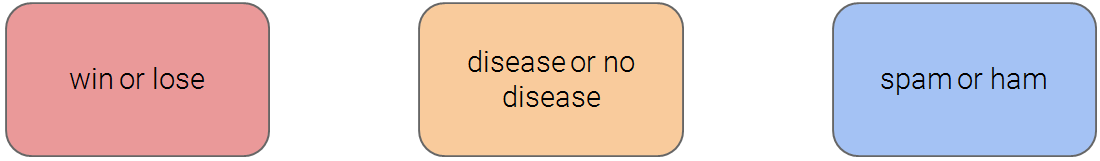
\includegraphics[scale=.5]{Bild1}
	    \end{figure}
	    However, the output of logistic regression is a continuous value in the range [0, 1], which we interpret as a probability – specifically,  P(Y=1|x)\\
	    \bigskip
	    In order to classify – that is, to predict a 1 or 0 – we pair our logistic model with a decision rule, or threshold.
	\end{frame}
	
	
	
	\begin{frame}{Thresholds}
	    Given an observation x, the following decision rule outputs 1 or 0, depending on the probability that our model assigns to x belonging to class 1.\\
	    \bigskip
	    Example for T = 0.5:
	    \begin{equation*}
	        classify(x)  =\left\{\begin{array}{cc}
	            1, &  P(Y=1|x) \geq 0.5 \\
	            0, &  P(Y=1|x) < 0.5
	        \end{array}\right.
	            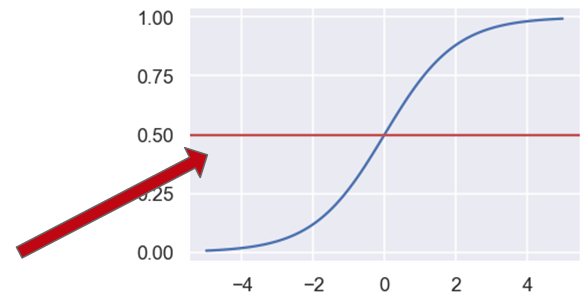
\includegraphics[scale=.25]{Bild2}
	    \end{equation*}
	    \begin{itemize}
	        \item Note: We don’t need to set our threshold to 0.5. Depending on the type of errors we want to minimize, we can increase or decrease it.
	        \begin{itemize}
	            \item 0.5 is the default in scikit-learn’s LogisticRegression, though.
	        \end{itemize}
	        \item Logistic regression paired with a decision rule is a classifier.
	    \end{itemize}
	\end{frame}
	
	
	\begin{frame}{Thresholds}
	    Consider the single-feature logistic regression model from last lecture:
	    \begin{equation*}
	        P(Y=1|x) = \sigma (\theta_1 \cdot FG\_PCT\_DIFF)
	    \end{equation*}
	    Here, the blue line represents our modeled probabilities, and the red lines represent various thresholds.
	    \begin{figure}
	        \centering
	        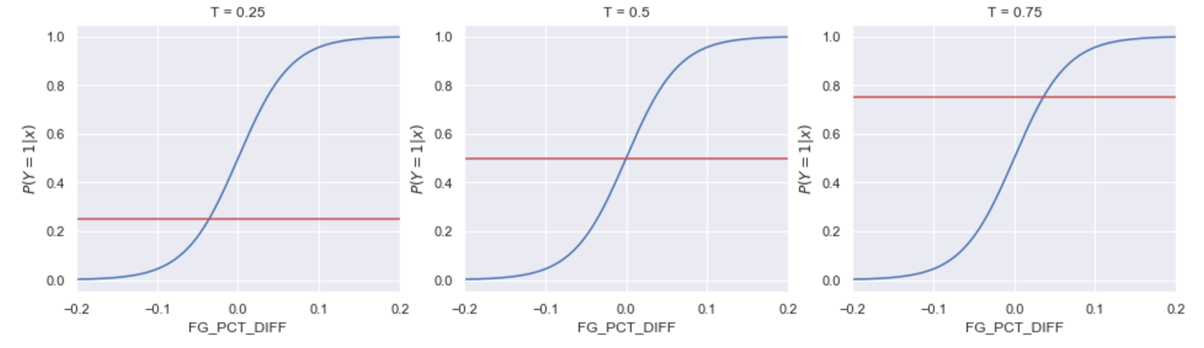
\includegraphics[scale=.5]{Bild3}
	    \end{figure}
	\end{frame}
	
	
	\begin{frame}{Thresholds in higher dimensions}
	    \begin{columns}
	        \begin{column}{.7\textwidth}
	                Our thresholds work the same way, even if our models have multiple features.\\
	                \bigskip
	                Suppose we fit a model with 2 features – FG\_PCT\_DIFF and PF\_DIFF – along with an intercept term.
	                \begin{align*}
	                    P(Y=1|x) = \sigma (\theta_0  + \theta_1 \cdot FG\_PCT\_DIFF + \theta_2 \cdot PF\_DIFF)
	                \end{align*}
	        \end{column}
	        
	        
	        \begin{column}{.4\textwidth}
	                \begin{figure}
	                    \centering
	                    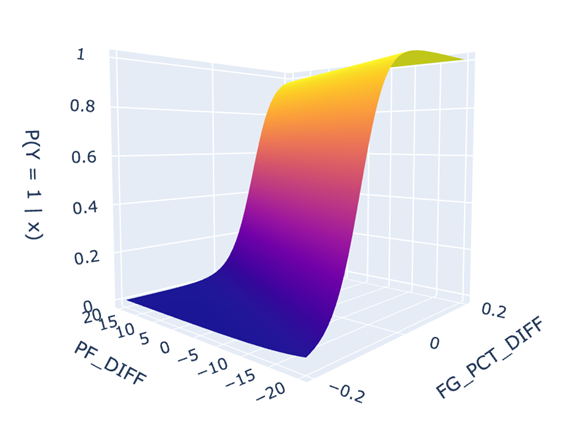
\includegraphics[scale=.5]{Bild4}
	                \end{figure}
	        \end{column}
	    \end{columns}
	\end{frame}
	
	
	\begin{frame}{Thresholds in higher dimensions}
	    \begin{columns}
	        \begin{column}{.7\textwidth}
	                Our thresholds work the same way, even if our models have multiple features.\\
	                \bigskip
	                Suppose we fit a model with 2 features – FG\_PCT\_DIFF and PF\_DIFF – along with an intercept term.
	                \begin{align*}
	                    P(Y=1|x) = \sigma (\theta_0  + \theta_1 \cdot FG\_PCT\_DIFF + \theta_2 \cdot PF\_DIFF)
	                \end{align*}
	                Any data point whose predicted probability is greater than 0.3 (above the plane) is classified as 1.
	        \end{column}
	        
	        
	        \begin{column}{.4\textwidth}
	                \begin{figure}
	                    \centering
	                    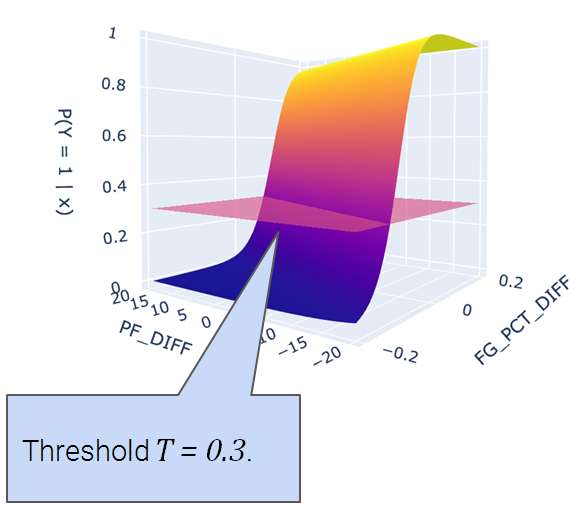
\includegraphics[scale=.35]{Bild5}
	                \end{figure}
	        \end{column}
	    \end{columns}
	\end{frame}
	
	
	
	\begin{frame}{From probabilities to labels}
	    \begin{columns}
	        \begin{column}{.7\textwidth}
	                With different thresholds, we get different predictions.
	                \begin{itemize}
	                    \item Everything above the red line is classified as 1, and everything below is classified as 0.
	                    \item The larger we make T, our threshold, the fewer observations are classified as 1.
	                    \begin{itemize}
	                        \item The “standard” is higher.
	                    \end{itemize}
	                \end{itemize}
	                \begin{figure}
	                    \centering
	                    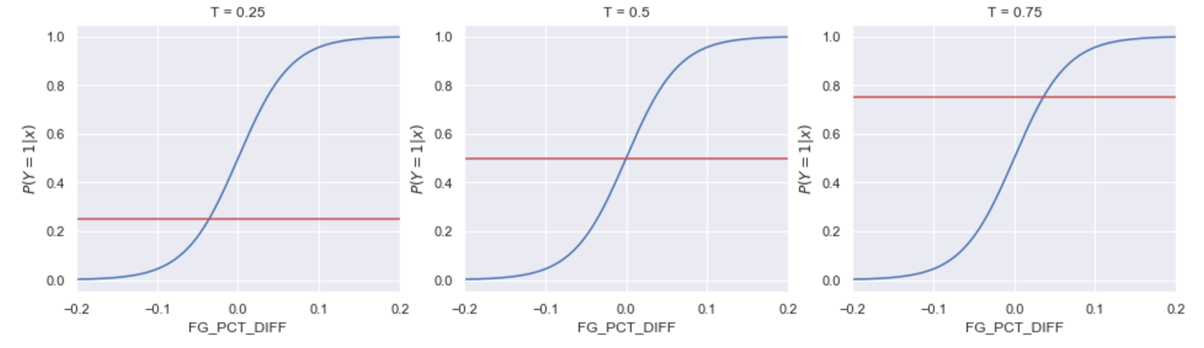
\includegraphics[scale=.5]{Bild3}
	                \end{figure}
	        \end{column}
	        
	        
	        \begin{column}{.4\textwidth}
	                \begin{figure}
	                    \centering
	                    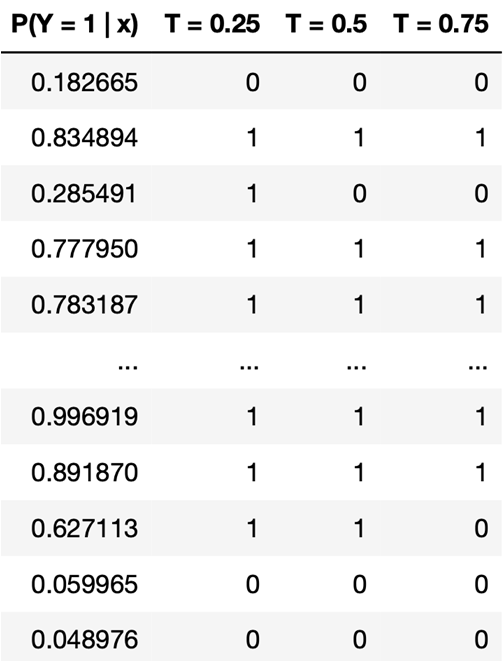
\includegraphics[scale=.5]{Bild6}
	                \end{figure}
	        \end{column}
	    \end{columns}
	\end{frame}
	
\end{document}